\section{Используемые технологии и приёмы программирования}

Важным этапом разработки любого программного средства является выбор подходящих
технологий разработки. При их выборе следует в первую очередь опираться на
требования к разрабатываемому программному средству и его особенности, связанные
с предметной областью.

В данном разделе будет приведено описание программной платформы,
используемых при разработке, и базы данных, применяемой в программе, а также
изложен подход, применяемый к проектированию архитектуры приложения.

\subsection{Фреймворк Qt}
\label{sec:qt}

Для обеспечения кроссплатформенности и упрощения разработки был выбран
популярный кроссплатформенный инструментарий разработки Qt и язык
программирования C++.

Qt позволяет запускать написанное с его помощью ПО в большинстве современных
операционных систем путём простой компиляции программы для каждой ОС без
изменения исходного кода. Он также включает в себя все основные классы, которые
могут потребоваться при разработке прикладного программного обеспечения, начиная
от элементов графического интерфейса и заканчивая классами для работы с сетью,
базами данных и XML. Qt выполнен в объектно-ориентированном стиле, легко
расширяем, обладает богатой документацией и активным сообществом. Графический
интерфейс, созданный с помощью Qt, корректно выглядит на всех поддерживаемых
операционных системах.

В отличие от большинства библиотек, Qt вносит некоторые расширения в синтаксис
C++ путем использования \moc{} — предварительной системы
обработки исходного кода. Благодаря данному обработчику реализована
сигнально-слотовая система, являющаяся ключевой особенностью Qt. \moc{}
преобразует лаконичный синтаксис сигналов и слотов в код на C++. Этот подход
в сочетании с богатой встроенной коллекцией классов значительно упрощает
процесс разработки. 

В Qt слоты и сигналы используются для коммуникации между объектами. Сигнал ---
это уведомление об определённом событии, а слот --- это функция, которая
вызывается в качестве ответа на определённый сигнал. Сигналы и слоты можно
связывать между собой, реализуя таким образом взаимодействие между различными
модулями программы. Техника, реализованная в Qt, является своего рода
синтаксическим сахаром для функций обратного вызова, которые как раз применяются
в таких случаях. Однако тесная интеграция данной системы со стандартными
классами фреймворка и лаконичный синтаксис позволяет полностью забыть о callback
и быстро создавать сложные пользовательские интерфейсы, многопоточные приложения,
приложения для работы с сетью, имеющие гибкую и легко расширяемую архитектуру.
Во некоторых случаях сигнально-слотовая система позволяет избежать ручной
реализации многопоточности, что уменьшает количество мест в коде 
для сложно обнаруживаемых ошибок, присущих многопоточным приложениям.

На рисунке \ref{fig:slots_signals} представлена схема связи между объектами и
синтаксис соединения сигналов и слотов в Qt. Как видно из иллюстрации, один и
тот же сигнал signal1 у объекта Object1 может быть связан с несколькими слотами
(связь <<один-ко-многим>>), аналогично несколько различных сигналов могут быть
привязаны к одному слоту (связь <<многие-к-одному>>).

\begin{figure}[h!]
\centering
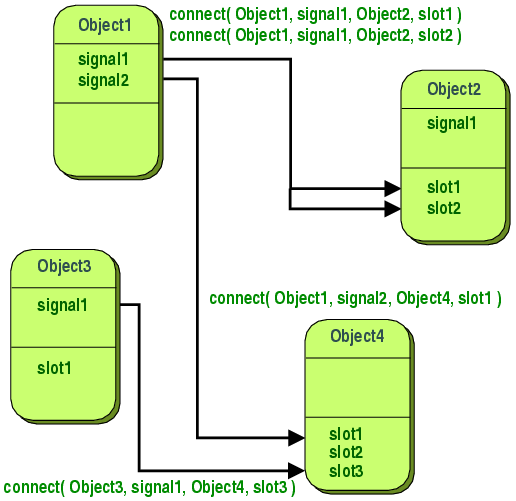
\includegraphics[scale = 0.6]{slots_signals.png}
\caption{Пример использования сигналов и слотов}
\label{fig:slots_signals}
\end{figure}

Модули библиотеки обеспечивают следующую функциональность:
\begin{itemize}
  \item создание элементов графического интерфейса;
  \item широкий набор классов для сетевого программирования;
  \item работа с базами данных;
  \item работа с XML и JSON;
  \item работа с мультимедиа;
  \item отображение веб-страниц с помощью движка WebKit;
  \item работа с технологиями ActiveX и COM в Windows;
  \item использование OpenGL. 
\end{itemize} 

При создании интерфейса приложения активно используется механизм QSS – Qt Style
Sheets, таблица стилей Qt, позволяющий полностью отделить визуальный дизайн от
разработки приложения.

QSS в значительной части был вдохновлён каскадными таблицами стилей CSS для
HTML, вследствие чего имеет похожий синтаксис. В частности, как и в CSS, в QSS
можно изменять форму, цвета, прозрачность элемента, а также визуальную реакцию
на события, такие, как нажатие кнопки, движение курсора над элементом и другие.
Стили можно присоединять как к отдельному компоненту так и ко всему приложению,
с помощью статического метода setStyleSheet(), имеющегося как у отдельных
виджетов, так и у класса QApplication. 

Qt Designer предоставляет возможность интеграции QSS-стилей, что упрощает их
разработку и тестирование.

Для компиляции файлов исходного кода, получающихся после обработки
системой \moc{}, можно использовать компиляторы GCC и MSVC. Для исключения
влияния особенностей компилятора на процесс сборки приложения принято решение
использовать компилятор GCC, имеющий версии под все целевые операционные
системы.

\subsection{Шаблон проектирования \mvc{}}

Достаточно часто в процессе разработки требуется вносить изменения в логику
работы программы. Любые видоизменения в логике влекут за собой изменения в
исходном коде. Как известно, при модификации исходного кода есть риск допустить
ошибку. Очевидно, что программирование без изменения исходного кода невозможно,
однако при проектировании архитектуры программы следует делать это так, чтобы
переписывать как можно меньше кода при внесении изменений в логику работы. Иными
словами, архитектура должна быть гибкой и расширяемой.

Паттерн проектирования --- это идея решения проблемы проектирования в
определенном, характерном контексте. Таким образом, само решение проблемы, то
есть реализация какого-либо паттерна на языке программирования, все еще является
задачей для разработчика, однако шаблон определяет некоторые аспекты отношения и
взаимодействия между классами и объектами, снижая сложность разработки.

Шаблон проектирования \mvc{} --- это популярный подход к построению архитектуры
приложения, когда модель приложения, интерфейс и взаимодействие с пользователем
разделены на три отдельных компонента таким образом, чтобы модификация одного из
компонентов оказывала минимальное воздействие на остальные (рисунок
\ref{fig:mvc}).

Основная цель применения этой концепции состоит в отделении модели от её
представления. За счет такого разделения повышается возможность повторного
использования кода. Наиболее полезно применение данной концепции в тех случаях,
когда пользователь должен видеть те же самые данные одновременно в различных
контекстах. Например, некоторые данные могут быть одновременно представлены в
виде электронной таблицы, гистограммы и круговой диаграммы.
Данный подход также упрощает совместную разработку, так как позволяет каждой
команде разработчиков концентрироваться только на своей задаче.
Поэтому возможно добиться того, что программисты, занимающиеся разработкой
бизнес-логики (<<модели>> в терминах MVC), вообще не будут осведомлены о том,
какое представление будет использоваться.

\begin{figure}[h!]
\centering
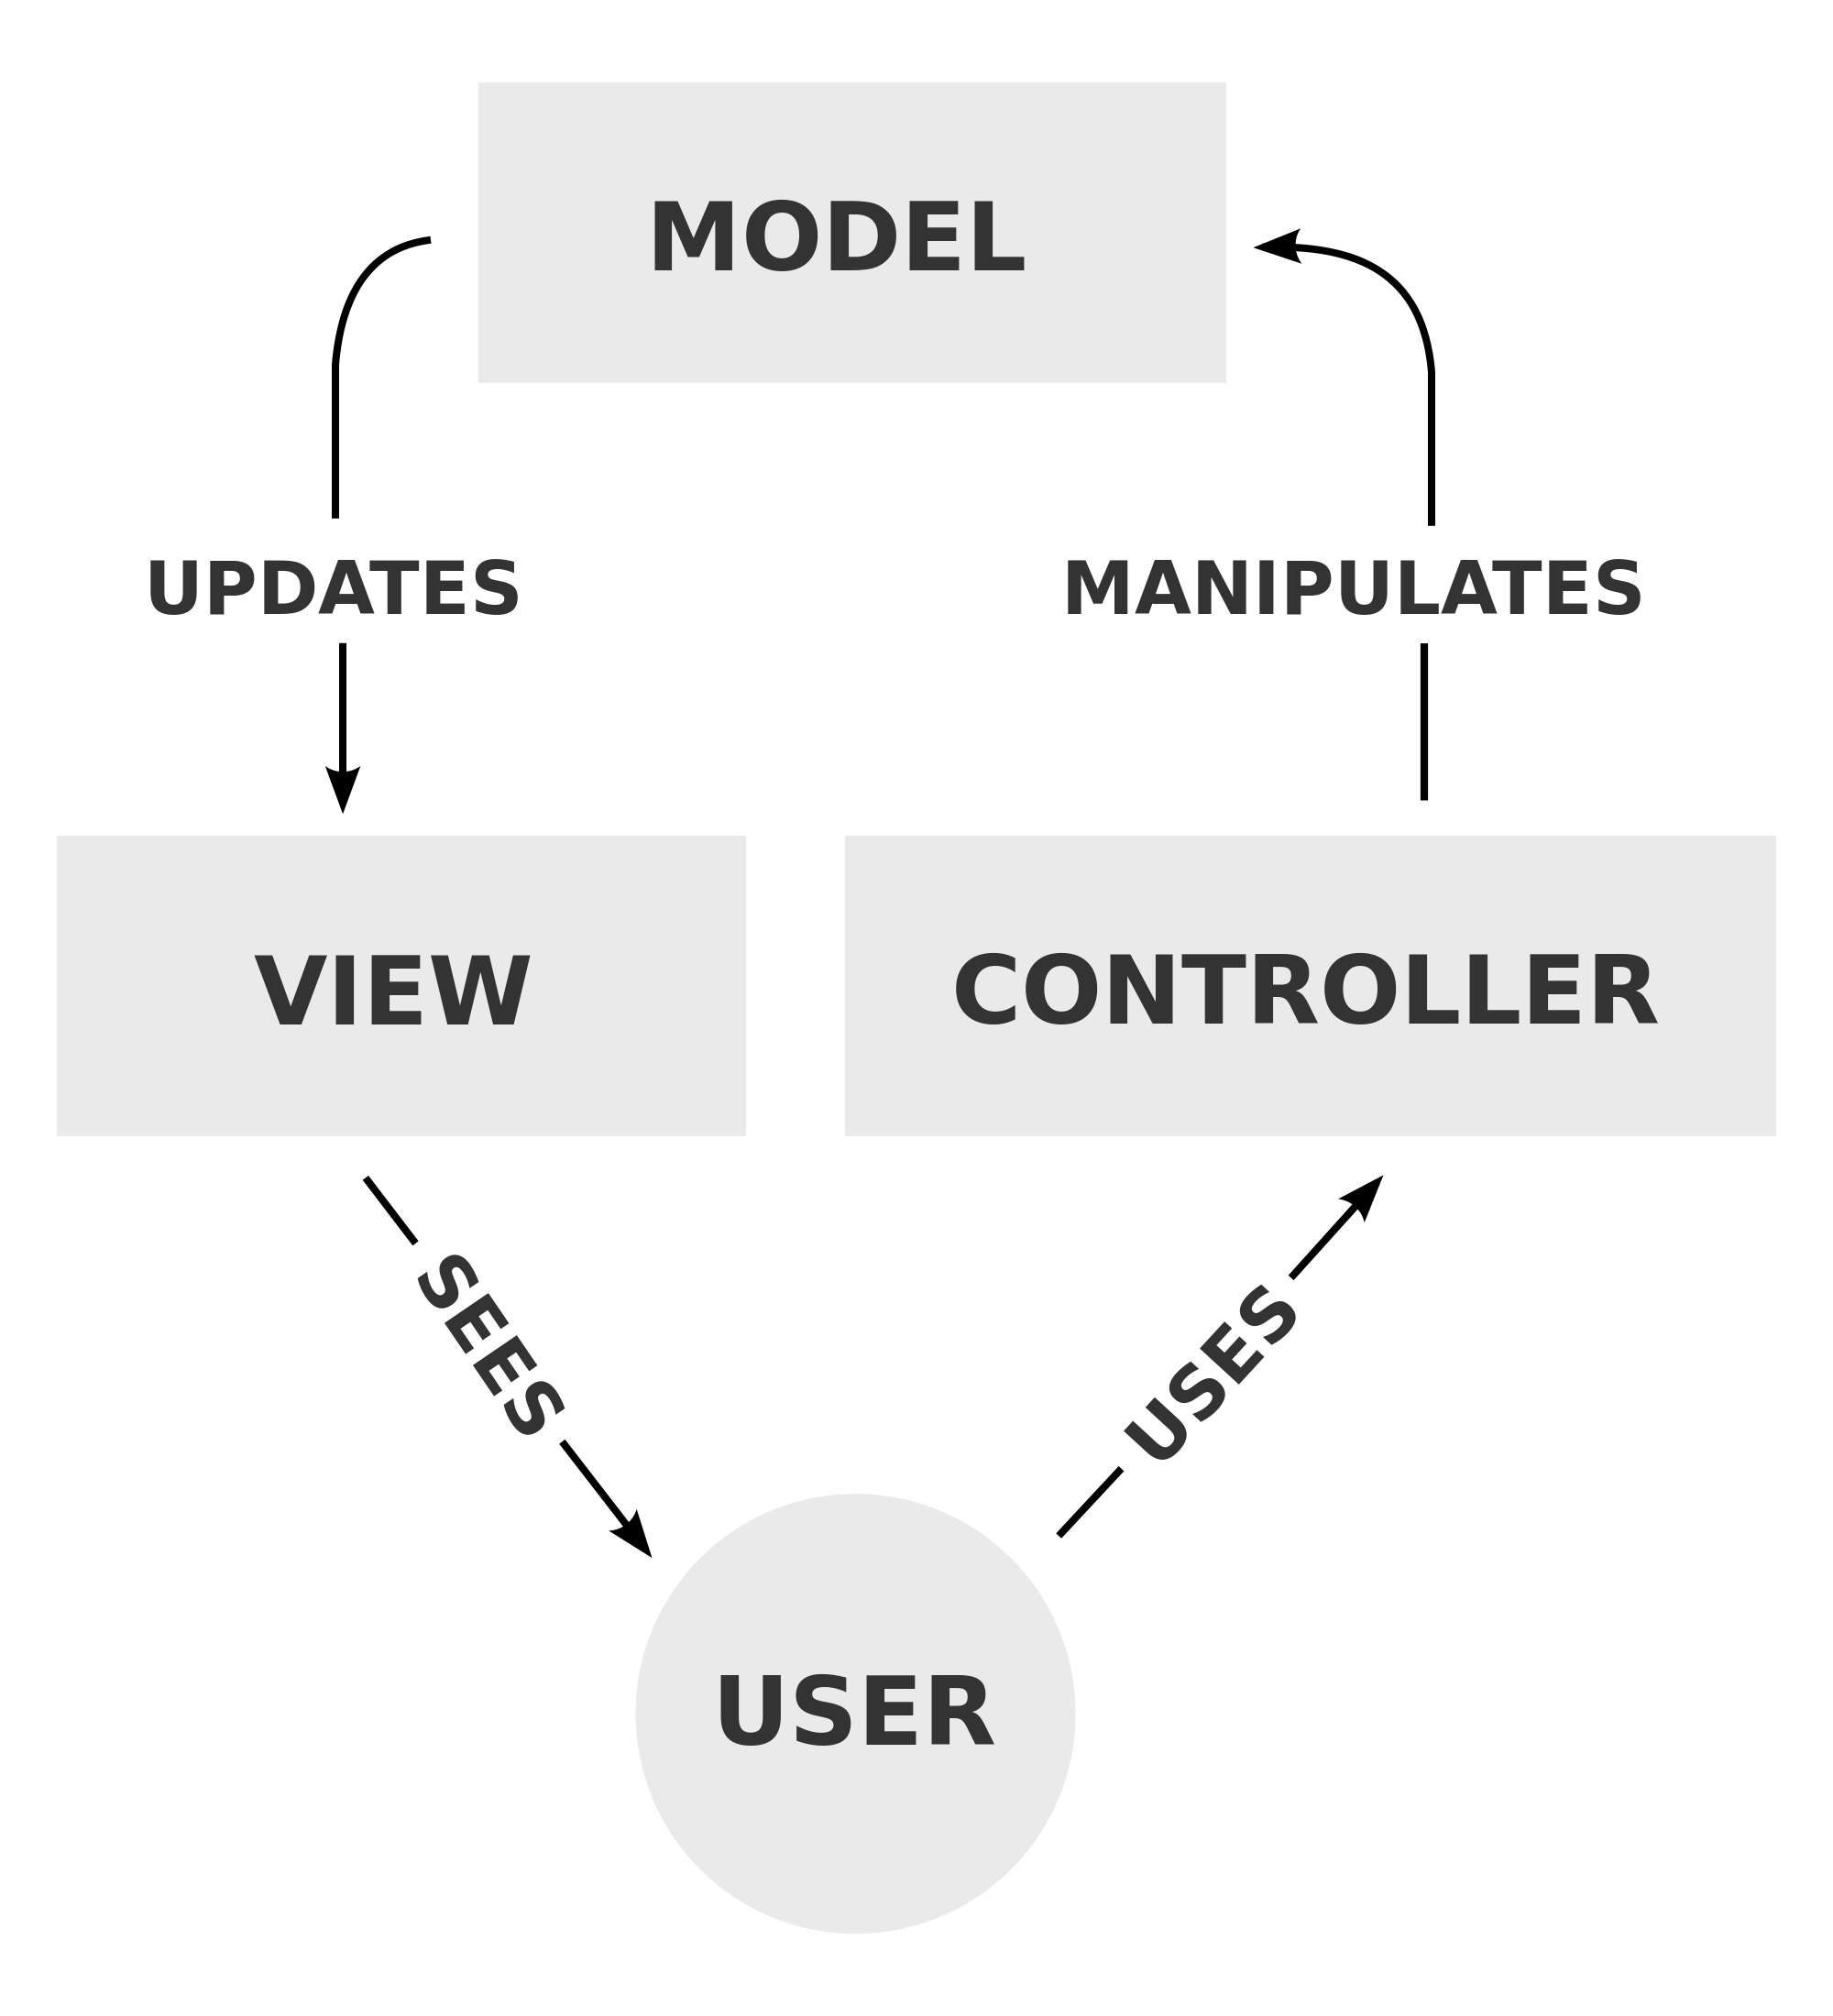
\includegraphics[scale = 0.15]{mvc.png}
\caption{Схема взаимодействия компонентов MVC}
\label{fig:mvc}
\end{figure}

При правильном применении \mvc{} существенно облегчает поддержку программы и
снижает затраты на изменение или добавление функциональности.

\subsection{База данных SQLite}
\label{sec:sqlite}
Процесс загрузки большого количества данных через запросы с API может занять
достаточно продолжительное время. Даже несмотря на возможность одновременной
загрузки данных и вывода уже загруженных, необходимо минимизировать расход
трафика и нагрузку на сеть в процессе работы с приложением путем кэширования
уже загруженных данных и периодического обновления кэша по мере появления новой
информации на сервере.

Для этих целей отлично подойдет встраиваемая реляционная база данных SQLite.
Данная база данных не использует клиент-серверную архитектуру, то есть не имеет
отдельно работающего процесса, взаимодействующего с клиентской программой и
базой данных, а предоставляет библиотеку, с которой программа компонуется. Таким
образом движок становится составной частью программы. SQLite хранит всю базу
данных в единственном файле, что уменьшает накладные расходы, время отклика и упрощает
программу.

Несколько процессов или потоков могут одновременно без каких-либо проблем читать
данные из одной базы. Запись в базу можно осуществить только в том случае, если
никаких других запросов в данный момент не обслуживается; в противном случае
попытка записи оканчивается неудачей, и в программу возвращается код ошибки.

SQLite отличается простотой использования и встраивания, в связи с чем активно
используется во многих популярных приложениях.




